\subsection{Disponibilidad vs Accesibilidad}
    
Como mencionamos en la introduccion de este capitulo, los datos pueden estar disponibles en la fuente original, pero no por
ello significa que estos sean accesibles.
Los retos a los que nos encontramos con los datos crudos, directos de la fuente de origen, son los siguientes:
    
    \begin{itemize}
        \item \textbf{Localizacion}. Los datos se encuentran disponibles en portales de datos abiertos organizados 
        y estructurados, normalmente se necesita una tarea de busqueda y seleccion
        a veces complicada. Aunque las empresas ponen cada vez mas de su parte en ofrecer una interfaz 
        agradable y funcional a los usuarios, esta tarea requiere de un trabajo de investigacion por parte del usuario,
        ya que posiblemente, debera buscar en distintos portales.
        \item \textbf{Accesibilidad}. Los datos suelen estan disponibles a traves de una interfaz de programacion 
        de aplicaciones (API) no facilmente interpretable por el usuario medio. Normalmente cuenta con 
        un documento que describe cada uno de los campos y valores que se presentan en el documento y como utilizar la API.
        \item \textbf{Interpretabilidad}. Usualmente los datos estan representados en un formato para ser procesado por 
        algun software, por lo que su lectura resulta complicada por el usuario medio, en el mejor de los casos, 
        estaran representados en una tabla y aun asi, sera muy dificil de extraer informacion.
        \item \textbf{Almacenamiento}. Los datos publicados son los mas recientes, por lo que no hay manera de obtener 
        un historico de los datos si no son almacenados periodicamente. Una vez extraidos los datos, el usuario debera 
        contar con una infraestructura que le permita almacenar los datos.
        \item \textbf{Automatizacion}. Este proceso tiende a ser arduo, por lo que sera necesario automatizarlo, de otra 
        forma el esfuerzo requerido por el usuario para extraer la informacion no le compensara.
         
    \end{itemize}
    
Por lo tanto, no podemos decir que estos datos sean accesibles de una forma util para el usuario medio.\\
 
\noindent\textbf{\textit{Aire Guru} }\\

Nuestra herramienta utiliza los datos de calidad del aire proporcionados por el ayuntamiento de Malaga en su portal de datos abiertos.\footnote{\url{https://datosabiertos.malaga.eu/}}\\
\begin{figure}[h]
    \centering
   \subfigure[Pagina principal]
    {\includegraphics[width=5.5cm  ]{OpenDataPortal}}
    \hfill
    \subfigure [Categoria medio ambiente]
       { 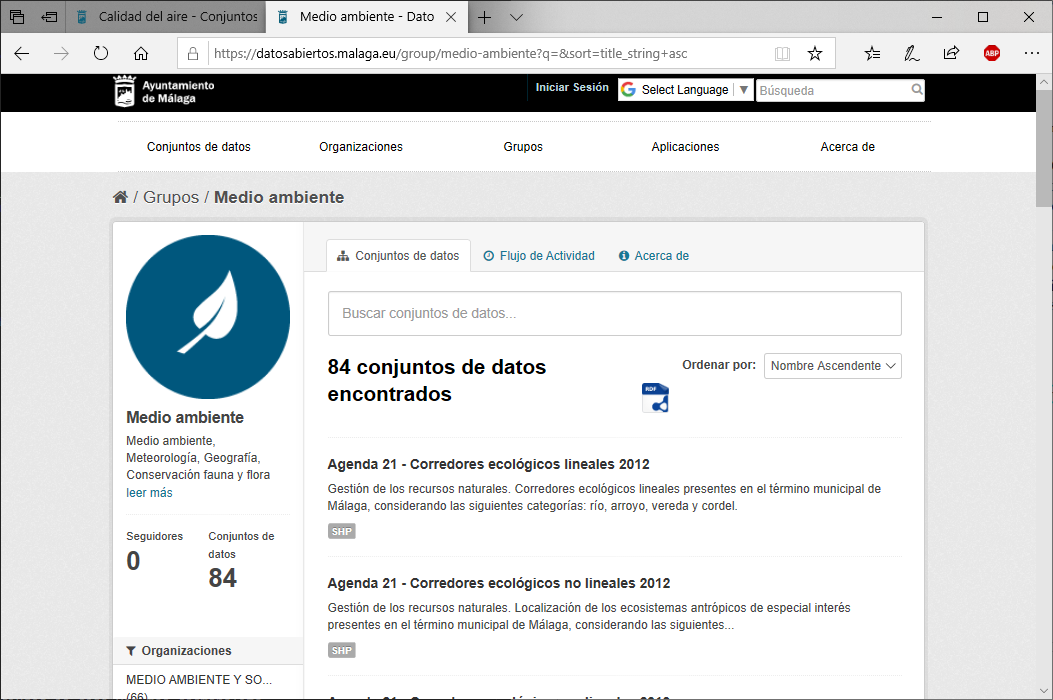
\includegraphics[width=5.5cm]{openDataPortalEnviromentCategory}}
  
  \caption{Open Data Portal Malaga}
    \end{figure}

    Este portal de datos ofrece una oferta de categorias representados por iconos, por lo que es necesario saber en que categoria se clasifica el conjunto
de datos, una vez que se accede a la categoria, tenemos una barra buscadora que nos permite insertar las palabras claves para buscar el conjunto de datos
deseado.\\
\begin{itemize}
    \item \textit{Evaluation}
\end{itemize}
El acceso a los datos no es directo ya que deberemos conocer la categoria en la que se ha clasificado por el ayuntamiento.
En este caso puede pulsarse sobre el enlace y este abrira los datos en una nueva pestana, por lo que la utilizacion de un sistema informatico
para la descarga de los datos no es extrictamente necesario.
Solo esta disponible en un formato.
Se actualiza cada hora, por lo que si queremos acceder a unos datos en concreto, deberemos repetir la operacion periodicamente.
Un factor importante de este conjunto de datos es saber la evolucion de la polucion por zonas, la extraccion de esta informacion no es posible
si no se realiza un almacenado de los datos.
